\chapter{绘制垫片立体图}
{\bfseries 知识目标}
\begin{itemize}
\item 掌握array命令
\end{itemize}

{\bfseries 技能目标}
\begin{itemize}
\item 能够运行array命令绘制结构相同的图样
\item 能够运行拉伸命令进行盘类块零件的三维建模
\end{itemize}

{\bfseries 本单提要}

本章通过完成垫片立体图的绘制,使读者能够掌握array命令的使用,进一步巩固拉伸命令的使用。图\ref{fig:tiaoyafadianpian}所示即为本章要完成的任务。
\noindent
\begin{figure}[htbp]
\centering
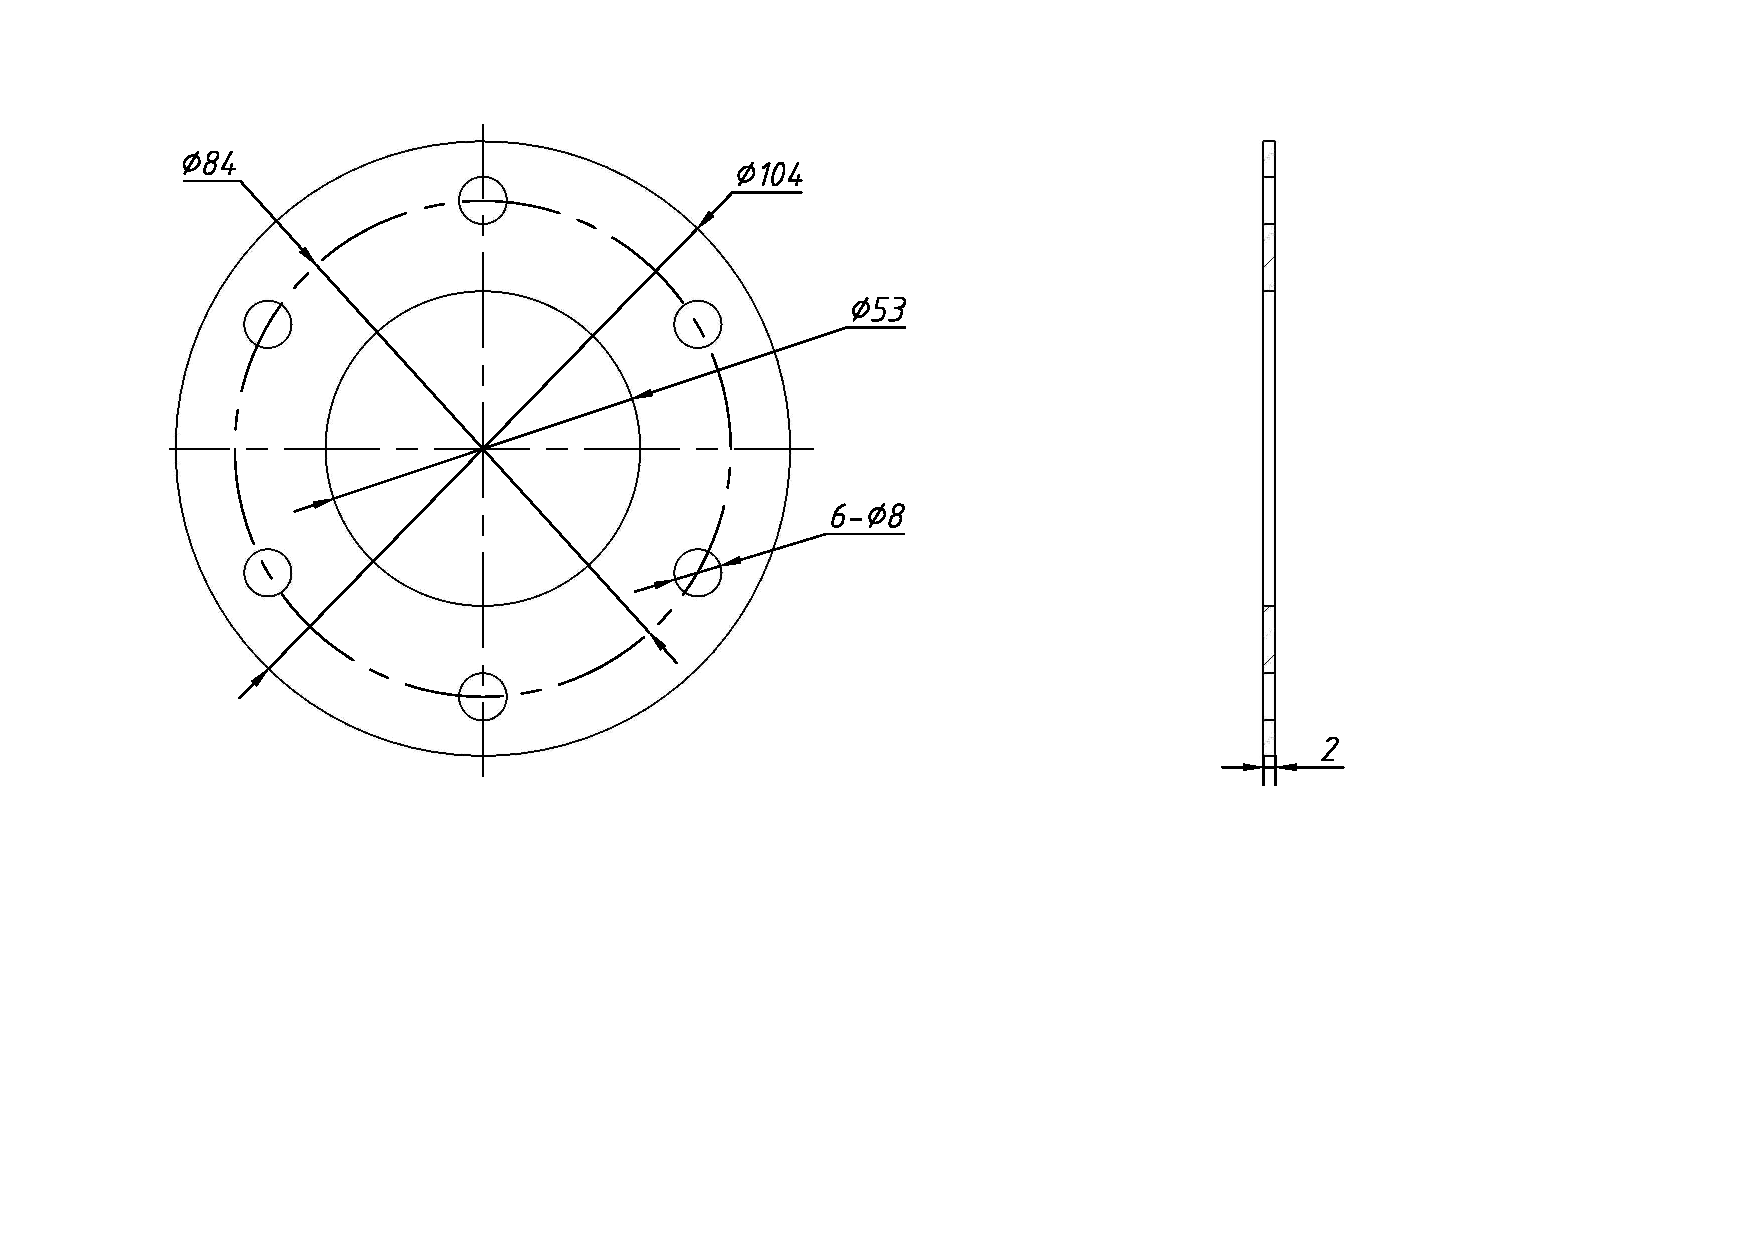
\includegraphics[scale=0.6]{tiaoyafadianpian.pdf}
\caption{垫片块零件图}\label{fig:tiaoyafadianpian}
\end{figure}

\endinput